\documentclass[presentation,t]{beamer}
\usetheme{EPCC}

% underline \emph{}
\usepackage{ulem}
\usepackage{listings}
\lstloadlanguages{C++,bash}
\lstset{basicstyle=\ttfamily,
  keywordstyle=\color{blue}\ttfamily,
  stringstyle=\color{red}\ttfamily,
  commentstyle=\color{magenta}\ttfamily,
  morecomment=[l][\color{magenta}]{\#},
  emphstyle=\underbar,
  language=C
}

\newcommand{\code}[1]{\lstinline!#1!}

% \usepackage{tikz}
% \usetikzlibrary{backgrounds,fit,calc,shapes,arrows,through,decorations.pathmorphing}
\newcommand{\thumb}[1]{
  \vfill{}
  % \hfill
  \begin{beamercolorbox}{fg=black}
    \begin{columns}[c,onlytextwidth]
      \begin{column}{0.07\textwidth}
        
\includegraphics[width=1em]{thumbs_up}
      \end{column}
      \begin{column}{0.93\textwidth}
        #1
      \end{column}
    \end{columns}
    % \end{block}
  \end{beamercolorbox}
  % \hfill
}

\author{Rupert Nash\\ \url{r.nash@epcc.ed.ac.uk}}
\date{13 June 2018}
\title{C++ for numerical computing}

\AtBeginSection[]{%
  \begin{frame}{Outline}
    \tableofcontents[currentsection]
  \end{frame}}

\begin{document}

\frame{\titlepage}
\section{Introduction}
\begin{frame}{What this is not!}
  Writing efficient software, more than anything, requires you to
  choose an appropriate algorithmic approach for your problem. For
  lots on how to do this well, take Parallel Design Patterns next
  semester!

  Here we want to take a lower-level approach and talk about how to
  implement patterns efficiently using C++.
\end{frame}

\begin{frame}{What is ``numerical computing''?}
  Both HPC and data science, when you actually come to running a
  program, are about getting a large amount of data from memory to a
  core, doing something useful to it, and storing it again.
  \vfill
  This is why FORTRAN is still relevant! But it does force you to
  confront this all time.
  \vfill
  I've mentioned previously than C++ is all about building
  abstractions and composing them.

  \thumb{I will talk about a few today and give some suggestions
  of default rules}
\end{frame}

\section{Containers}
\begin{frame}{STL Containers}
  The standard library has 13 container template classes, but we'll
  only touch on a few.

  \begin{itemize}
  \item \code{vector} - a dynamically sized contiguous array
  \item \code{array} - a statically size contiguous array
  \item \code{list}/\code{forward_list} - a doubly/singly linked list
  \item \code{set} / \code{map}
    
  \end{itemize}

\end{frame}

\begin{frame}[fragile]{vector - your new best friend}
  You will be using this a lot, because the elements are contiguous in
  memory.
\begin{lstlisting}
#include <vector>

std::vector<int> primes(unsigned n) {
  std::vector<int> ans;
  for (auto i=2; i<n; ++i) {
    if (isprime(i))
      ans.push_back(i);
  }
 return ans
}
\end{lstlisting}
  \thumb{Use by default - data locality often wins over algorithmic complexity}
\end{frame}

\begin{frame}{vector - your new best friend}
  Supports:
  \begin{itemize}
  \item copy
  \item move
  \item random element access by index
  \item resize (and pre-reserving memory)
  \item element insertion
  \item element deletion
  \end{itemize}
  Note that when it destructs, contained elements will also be
  destroyed (i.e. it \emph{owns} them).
  
  Also be aware that resizes may force reallocation and copying!
\end{frame}

\begin{frame}[fragile]{array}
  \begin{itemize}
  \item Contiguous in memory but the size is fixed at compile time.

  \item Almost like a vector, but you can't change the size.

  \item Only difference is construction:
  \end{itemize}

\begin{lstlisting}
#include <array>
typedef std::array<int, 3> GridPoint;

GridPoint p1 = {1,2,3};
GridPoint p2{{5,2,5}};
// horrible extra brace can go in C++14
std::cout << p2.size() << std::endl; \\ 3

\end{lstlisting}

\end{frame}

\begin{frame}{list (and forward\_list)}
  \begin{itemize}
  \item Almost always implemented as a doubly (singly) linked list.
  
  \item Elements are allocated one by one on the heap.  Traversal
    requires pointer chasing.

  \item Fast element insertion and deletion (if you don't have to look
    for the element!)
  \end{itemize}
  \thumb{Use when you will be adding and removing from ends a lot and
    the contained objects are expensive to copy/move. Consider
    converting to \code{vector} if you have a build/access pattern.}
\end{frame}

\begin{frame}{set and map}
  \begin{itemize}
  \item These are associative containers implemented as sorted data
    structures for rapid search.

  \item \code{set} is just a set of keys, \code{map} is a set of
    key/value pairs (types can differ).
  
  \item You must have defined a comparison function for the key type.
  \end{itemize}
  
  \thumb{Use if you either 
    \begin{itemize}
      \item have a large key space that mostly lacks value, or
      \item will be looking up unpredictable values a lot or
        frequently adding/removing values.
      \end{itemize}
    }
\end{frame}

\begin{frame}{set and map}
  For example, describing your communication pattern between MPI ranks
  with a domain decomposed problem
  \begin{center}
  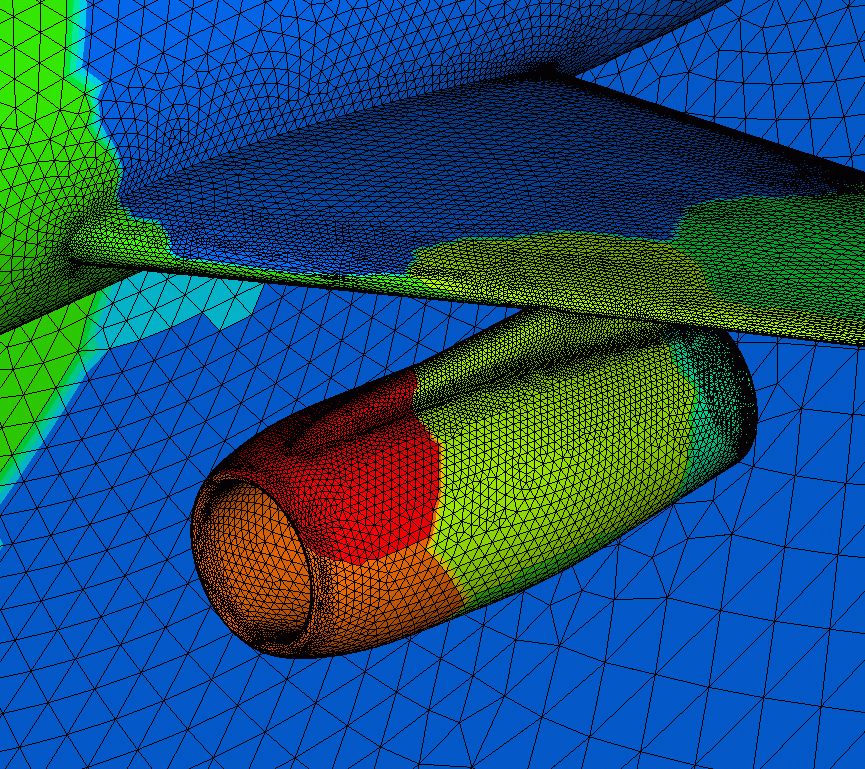
\includegraphics[width=0.7\textwidth]{domain_decomp}
\end{center}
\end{frame}

\begin{frame}[fragile]{set and map}
\begin{lstlisting}
std::map<int, BoundaryComm> rank2comms;
for (auto p =0; p != MPI_COMM_SIZE; ++p) {
  if (ShareBoundaryWithRank(p)) {
    rank2comms[p] = BoundaryComm(my_rank, p);
  }
}
// later
for (auto iter = rank2comms.begin(),
          end = rank2comms.end();
     iter != end; ++iter) {
  auto& bc = iter->second;
  bc->SendData(local_data);
}
\end{lstlisting}
\end{frame}
\section{Iterators}
\begin{frame}[fragile]{Iteration}
C programmers are used to:
\begin{lstlisting}
unsigned n = 100;
double* data = GetData(n);
for (auto i=0; i != n; ++i) {
  data[i] *= 2;
}
\end{lstlisting}

More old-skool C programmers will prefer this:
\begin{lstlisting}
unsigned n = 100;
double* start = GetData(n);
double* stop = start + n;
for (auto ptr = start; ptr != stop; ++ptr) {
  *ptr *= 2;
}
\end{lstlisting}
\end{frame}
\begin{frame}{Iteration}
These three humble pointers can implement the concept of traversing
every element in the array (in order).
\vfill
They also model the concept of an \emph{iterator} which is a vital for
using the standard library effectively.
\vfill
There are a few different categories of iterator (forward, backward,
random, etc) but they all can traverse the elements of something
(e.g. a container, data in a file, input from keyboard) and provide
access to them.
\end{frame}

\begin{frame}[fragile]{Iteration}
  A C++ equivalent of the previous might be:
\begin{lstlisting}
std::vector<double> data = GetData(n);
for (std::vector<double>::iterator iter 
                                = data.start();
     iter != data.end();
     ++iter) {
  *iter *= 2;
}
\end{lstlisting}
\pause
Or equivalently
\begin{lstlisting}
std::vector<double> data = GetData(n);
for (auto iter = data.begin();
     iter != data.end(); ++iter) {
  *iter *= 2;
}
\end{lstlisting}

%(I $\heartsuit$ \code{auto})
\end{frame}

\begin{frame}[fragile]{Er why?}
  What do we gain? \pause Separation of concerns!

  We can separate the data and how it's stored from the way we're
  traversing it, and also from the operations we apply to it.

  \pause
\begin{lstlisting}
template <class ItT>
void doubleInPlace(ItT start, ItT end) {
  for (auto iter = start; iter != end; ++iter)
    *iter *= 2;
}

std::vector<double> data = GetData(100);
doubleInPlace(data.begin(), data.end());

std::list<HugeMatrix> mats = GetMatrices();
doubleInPlace(mats.begin(), data.end());

\end{lstlisting}
\end{frame}

\begin{frame}{Container iterators}
  All the STL containers contain two iterator types, for example:
  \begin{itemize}
  \item \code{std::list<char>::iterator} - instance must be
    non-\code{const} - get with \code{begin()} or \code{end()}.
  \item \code{std::list<char>::const_iterator} - if the instance is
    \code{const} you get one of these from
    \code{begin()}/\code{end()}, if non-const, you can get one with \code{cbegin()}/\code{cend}.
  \end{itemize}
  \vfill
  
  You can also get iterators from e.g. \code{std::map<KeyT,
    ValT>::find(search_key)}, which will give and iterator pointing to
  the element you want or to the \code{end()}.
  \vfill
  Note that an iterator pointing to the end is not valid!
  Dereferencing it may have undefined behaviour...
\end{frame}

\begin{frame}{Implementing your own iterator}
  To define your own iterator, you need to create a class with several
  overloads (exactly which one depends on the category of iterator you
  need).
  
  \begin{itemize}
  \item derefence operator (\code{*it}) - you have to be able to get a value
    (either to read or write)
  \item pre-increment (\code{++it}) - you have to be able to ``go to
    the next one'' \footnote{Why not post-increment? Because this has
      to return the value of \code{it} from \emph{before} it was
      incremented. This usually means a copy.}
  \item assigment - you need to bind it to name
  \item inequality comparison (\code{it != end}) - you need to know
    when you are done
  \end{itemize}
\end{frame}

\begin{frame}[fragile]{Range for loop}
  Any class instance with \code{begin()} and \code{end()} member
  functions that return iterators can be used in a range based
  for-loop.
\begin{lstlisting}
std::vector<int> primes = getPrimes(5);
for (auto p : primes) {
  std << p << " " << std::endl;
}
// 2 3 5 7 11 
\end{lstlisting}

Almost ``pythonic''?
\end{frame}

\begin{frame}[fragile]{Range for loop}
  The compiler will translate this for us into something approximating
  the following
\begin{lstlisting}
{
  auto&& _range = <range expression>; 
  for (auto _begin = _range.begin(),
            _end = _range.end();
       _begin != _end;
       ++_begin) { 
    <range declaration> = *_begin;
    <loop body> 
  }
}
\end{lstlisting}
\end{frame}

\begin{frame}[fragile]{Is there any overhead?}
  Going to quickly compare three implementations
  \begin{itemize}
  \item C-style array indexing
  \item Standard vector with iterator 
  \item Standard vector with range based for-loop
  \end{itemize}

\begin{lstlisting}
int main(int argc, char** argv) {
  int size = std::atoi(argv[1]);
  std::vector<float> data(size);
  for (auto& el: data)
    el = rand(1000);
  Timer t;
  scale(data.data(), data.size(), 0.5);
  std::cout << size << ", " 
            << t.GetSeconds() << std::endl;
}
\end{lstlisting}
\end{frame}

\begin{frame}{Results}
  \only<1>{
    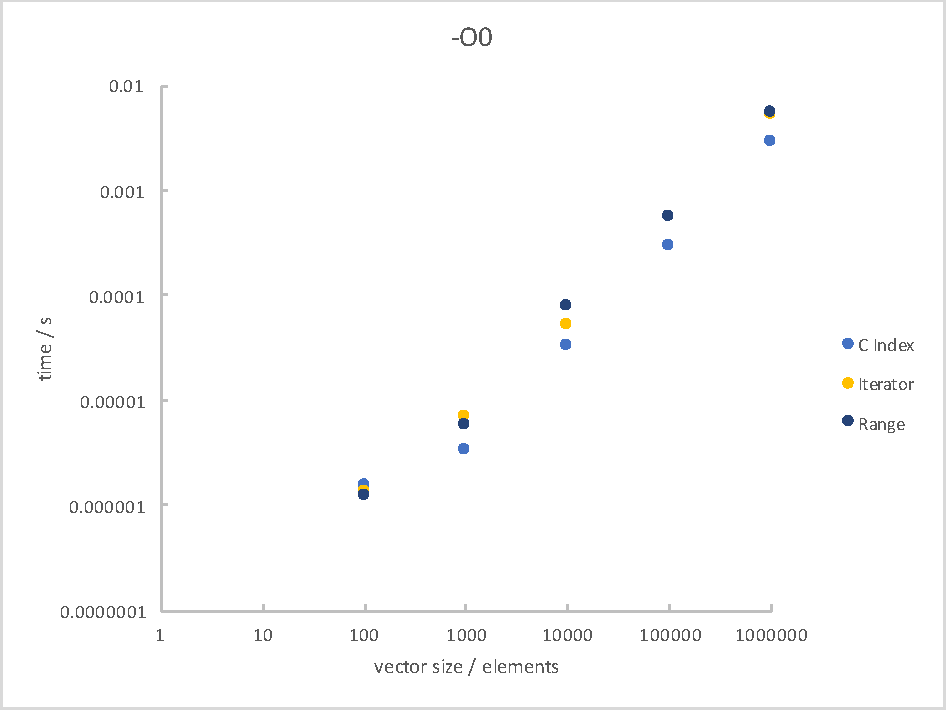
\includegraphics[height=\textheight]{looptests/O0.pdf}
  }
  \only<2>{
    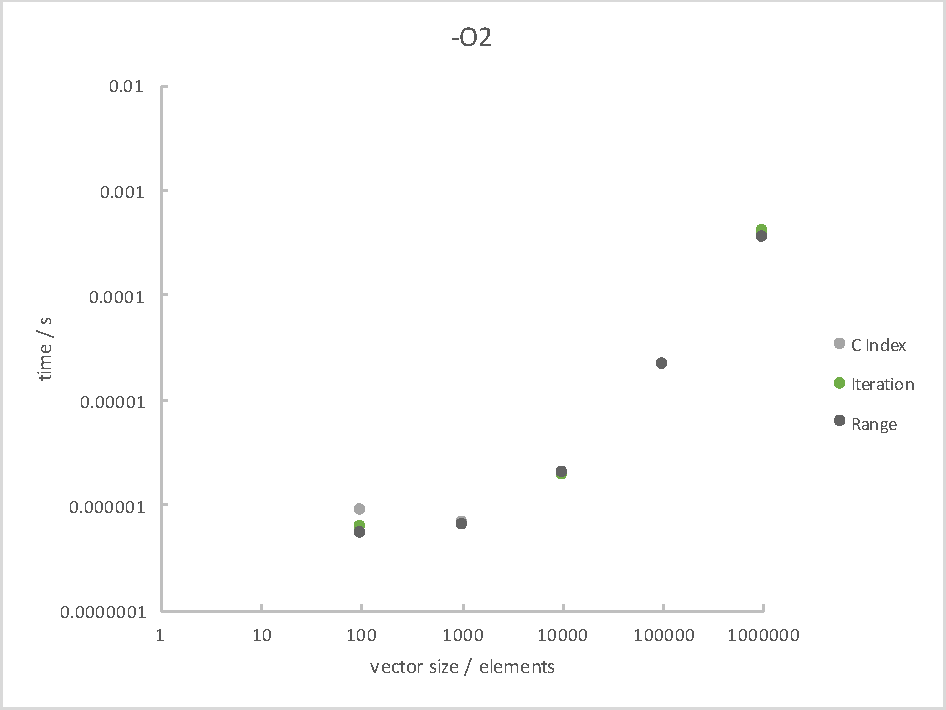
\includegraphics[height=\textheight]{looptests/O2.pdf}
  }
\end{frame}

\begin{frame}{Assembly}
  Just showing the main loops:
  \begin{columns}
    \begin{column}{0.5\textwidth}
      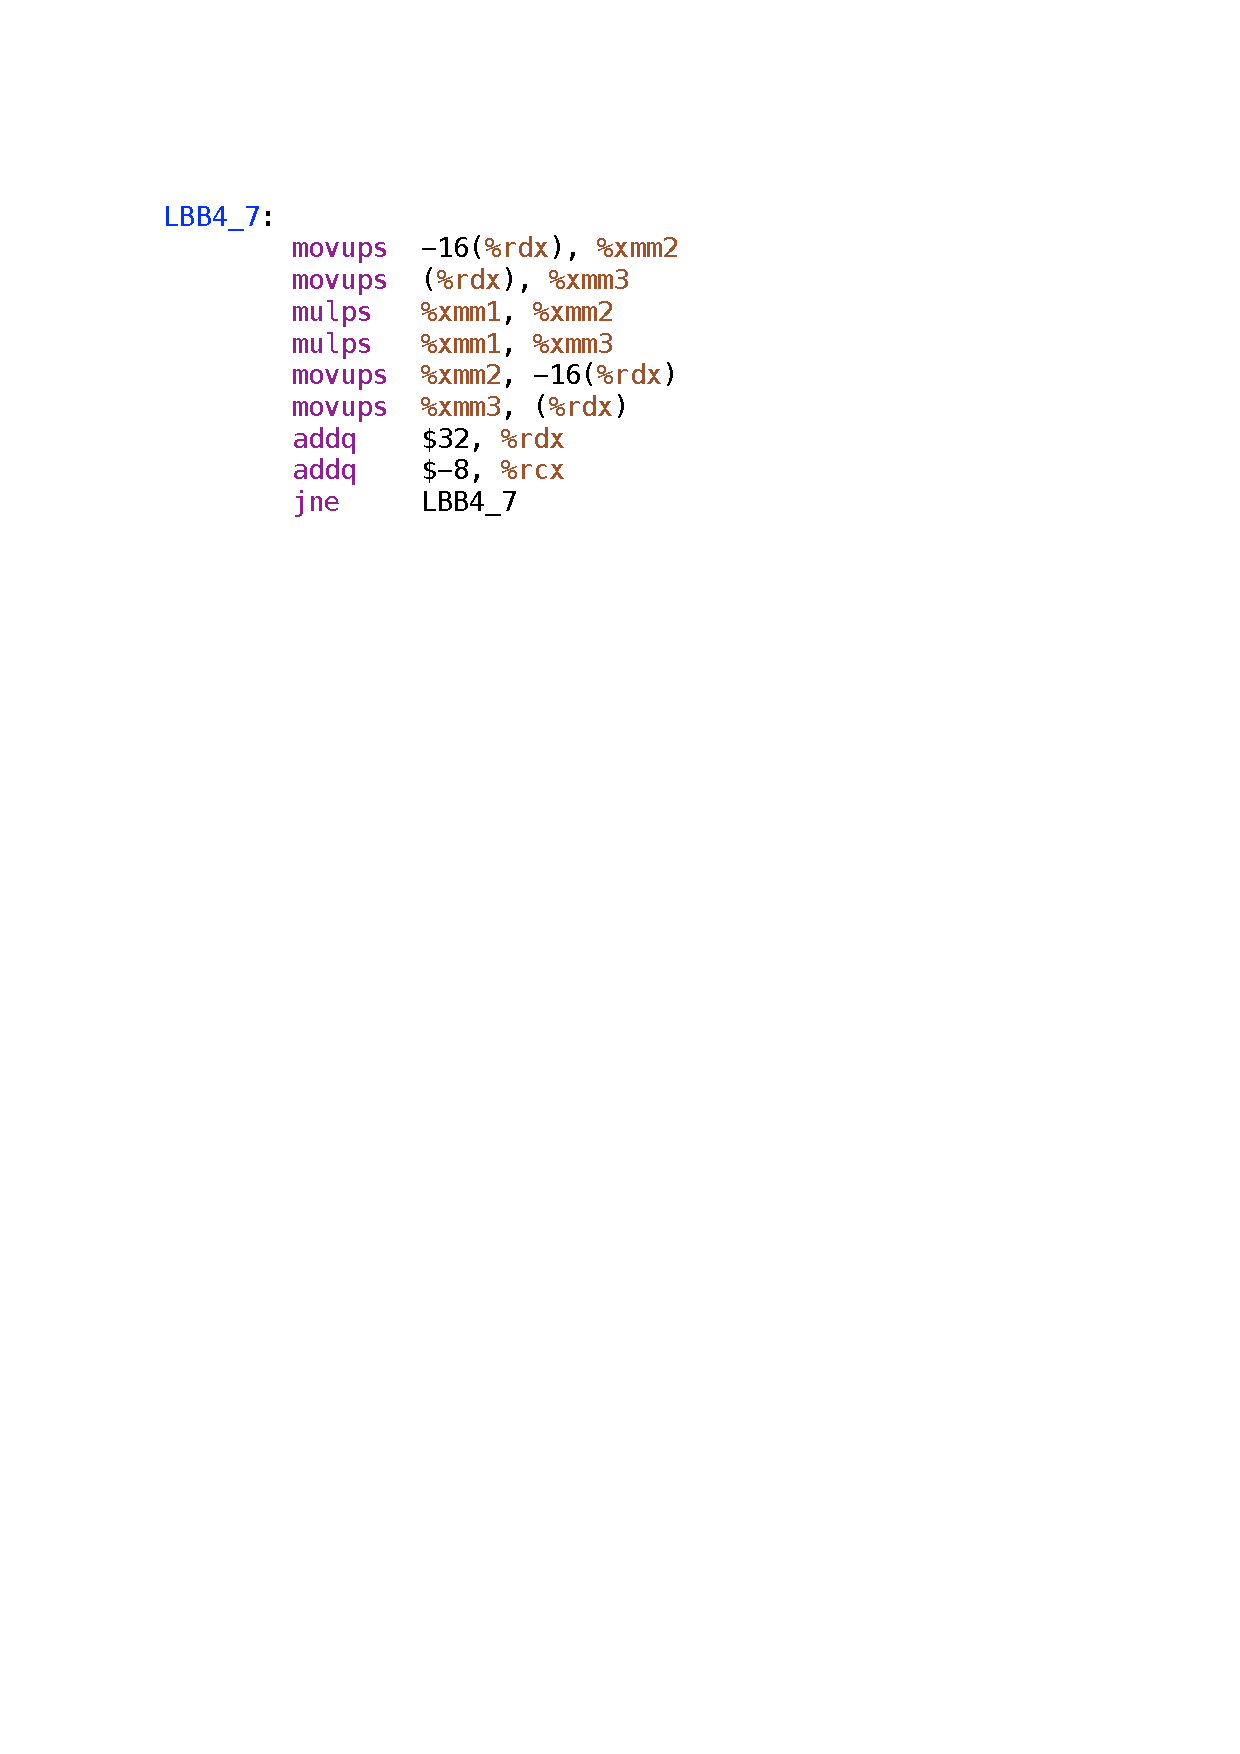
\includegraphics[width=\textwidth]{looptests/cstyleO2.pdf}
    \end{column} 
    \begin{column}{0.5\textwidth}
      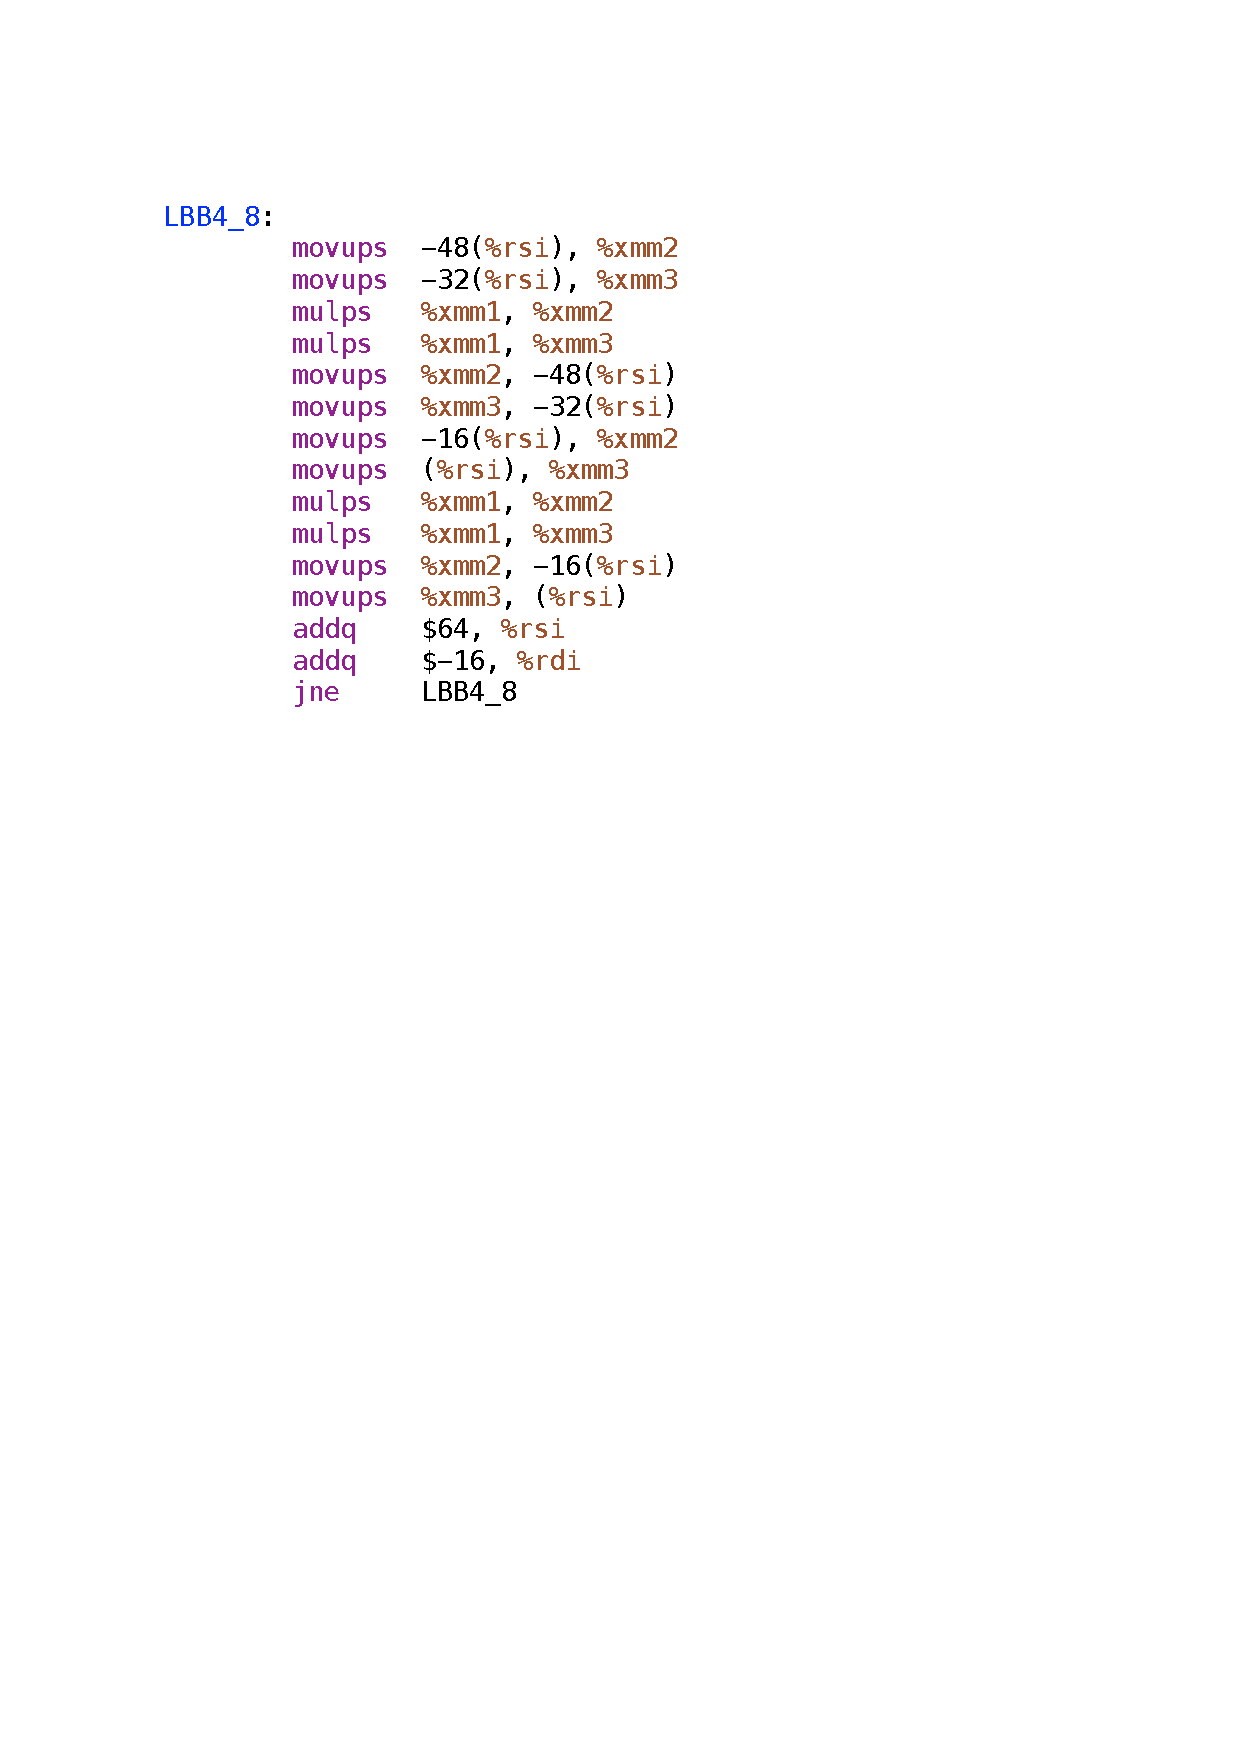
\includegraphics[width=\textwidth]{looptests/rangestyleO2.pdf}
    \end{column}   
  \end{columns}
\end{frame}

\section{Object oriented C++}
\begin{frame}
  Object oriented programming is one of the major paradigms supported
  by C++
  \begin{quote}OOP is based on the concept of ``objects'', which may
    contain data and code. A feature of objects is that an object's
    procedures can access and often modify the data of the object with
    which they are associated.
  \end{quote}
  
  We briefly covered how to create classes - today we'll go a little
  deeper.
\end{frame}

\begin{frame}{Inheritance}
  \begin{itemize}
  \item Inheritance is a method for deriving a new, related class from
    another one (called the base class, parent class, or super class).

  \item This relationship says that the derived object also \emph{is}
    an object of the base class too!
  
  \item The new class (derived, child, sub) has all the data and
    function members of its parent, but you can add new ones and
    \emph{override} existing ones.

  \item The derived class member functions can access the base class
    members that are public, but not the private ones. There is a
    third access specifier \code{protected} that allows derived
    classes to access the member.

  \item It's use should be minimal as you are promising to all
    subclasses that this interface will not change!
  \end{itemize}
\end{frame}

\begin{frame}[fragile]{Inheritance}
Suppose you had to process a lot of image files. You might start with
a JPEG file:
\begin{lstlisting}
class JpegFile {
  string _fn;
  int _nx, _ny;
  unique_ptr<char> _pixeldata;
public:
  JpegFile(string fn) : _fn(fn) {
     // read _nx/_ny/_ncols from header
    _pixeldata = new char[_nx*_ny*3];
    // decompress data from file
  }
  char& GetPixel(int x, int y) {
    return _pixeldata[x*_ny + y];
  }
};
\end{lstlisting}
\end{frame}

\begin{frame}{Inheritance}
  But then you have to add PNG, and GIF, and ...
  \pause
  
  Might want to do the same for each one, but:
  \begin{itemize}
  \item code duplication :(
  \item the types are totally unrelated :(
  \end{itemize}
\end{frame}

\begin{frame}[fragile]{Inheritance}
  So instead create a base class and several derived classes
\begin{lstlisting}
class ImageFile {
  string _fn;
protected:
  int _nx;
  int _ny;
  unique_ptr<char> _pixeldata;
public:
  ImageFile(string fn);
  char& GetPixel(int x, int y);
};
\end{lstlisting}
\end{frame}

\begin{frame}[fragile]{Inheritance}
  So instead create a base class and several derived classes
\begin{lstlisting}
class JpegFile : public ImageFile {
public:
  JpegFile(string fn) : ImageFile(fn) {
    // read _nx/_ny/_ncols from header
    _pixeldata = new char[_nx*_ny*3];
    // decompress data from file
  }
};

class PngFile : public ImageFile {
public:
  PngFile(string fn);
};

\end{lstlisting}
\end{frame}

\begin{frame}[fragile]{Pointers to base class}
One important thing to know is that a pointer to a derived class
(\code{JpegFile*}) is \emph{type compatible} with a pointer to the
base class (\code{ImageFile*}).

\begin{lstlisting}
JpegFile jpg("cat.jpg");
ImageFile* img = &jpg;
// also works with references
ImageFile& im_ref = jpg;
\end{lstlisting}

\end{frame}

\begin{frame}{Dynamic polymorphism}
  \begin{itemize}
  \item What if we have some behaviour, like writing the image data to
    file, that varies between the subclasses?

  \item We ideally want to have a uniform interface and when we call
    it as run time the pointer-to-base knows which subclass method to
    call.

  \item Enter virtual functions!
  \end{itemize}
\end{frame}

\begin{frame}[fragile]{Dynamic polymorphism}
\begin{lstlisting}
class ImageFile {
public:
 virtual void Write(string fn} = 0;
};

class JpegFile : public ImageFile {
public:
    virtual void Write(string fn} {
      // write header
      // compress + write data
    }
};
ImageFile* img = new JpegFile("cat.jpg");
img->Write("notdog.jpg");
\end{lstlisting}
\end{frame}

\begin{frame}{How does this work?}
  \begin{itemize}
  \item Through a virtual function table.

  \item Each class has a static table of function pointers that point
    to the code of its virtual functions.

  \item Each instance of the class has a pointer to the table that
    belongs to its actual class (filled in by the compiler in the
    constructor).

  \item To call, the object's ``vtable'' pointer is followed, the
    offset for the method added, and the function called by
    pointer. Clearly slower than a simple function call by
    compile-time constant! Worse it make inlining of the function
    impossible.

  \item You really don't want to use virtual functions in an inner
    loop!

    (By all means use them outside!)
  \end{itemize}
\end{frame}
% inheritance
% polymorphism
% pitfalls - object soup
% alternative
\end{document}
